\documentclass[8pt]{beamer}

\setbeamertemplate{background canvas}[vertical shading][bottom=cyan!10,top=blue!10]

\usetheme{Warsaw}
\usefonttheme[onlysmall]{structurebold}

% pour le fichiers .pdf
\usepackage{graphicx}
\usepackage{color}
% pour les fichiers .png
% \usepackage{pgf,pgfarrows}
% \usepackage{pgf,pgfarrows}
\usepackage{amsmath,amssymb}
\usepackage{textcomp}
\usepackage{multitoc}
\usepackage{mdwtab}
\setbeamercovered{dynamic}
\DeclareMathOperator*{\argmin}{argmin}

\title[OpenTURNS modules development]{OpenTURNS modules development}
\author[OpenTURNS Consortium, 2019]
{
  Trainer : Sofiane Haddad\\
  Airbus \\
  sofiane.s.haddad@airbus.com
}



\date[Mai 14-17th 2011]
{
  Developers training \\

  \begin{center}
    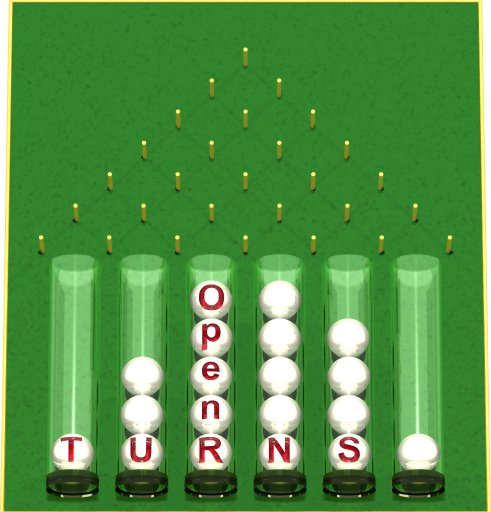
\includegraphics[height=2cm]{logoOT.jpg}
  \end{center}
}

\subject{OpenTURNS Developers Training}

% \part<presentation>{Corps de presentation}


\begin{document}

\frame{\titlepage}

% necessaire pour la table des matieres
\part{Main part}

% table des matieres
\begin{frame}
  \frametitle{OpenTURNS modules development}
  \tableofcontents[part=1]
\end{frame}
%%%%%%%%%%%%%%%%%%%%%%%%% 
% The OpenTURNS package %
%%%%%%%%%%%%%%%%%%%%%%%%% 
\section[OpenTURNS modules]{OpenTURNS modules}
%%%%%%%%%%%%% 
% The tools %
%%%%%%%%%%%%% 
\begin{frame}
  \frametitle{OpenTURNS modules}
  \begin{block}{Objectives}
    OpenTURNS is a growing system developed by a small team. A constant problem is to assess the stability of the whole product, and in order to achieve this goal we introduced a notion of module, in order to insulate a core library dedicated to the definition of the abstract data model and to propose all the specific algorithms as optional modules. The core would evolve quite slowly, insuring its robustness, whereas the modules would have a more dynamic development model.\\
    Another key objective is to provide a way to extend the existing platform with functionalities developed by teams that are reluctant to adopt the OpenTURNS development process. Within the module, the development team can adopt any coding rule or programming language he want, as long as the OpenTURNS interface is respected as well as the objects lifecycle.
  \end{block}
\end{frame}
\begin{frame}
  \frametitle{OpenTURNS modules}
  \centering \resizebox{!}{4cm}{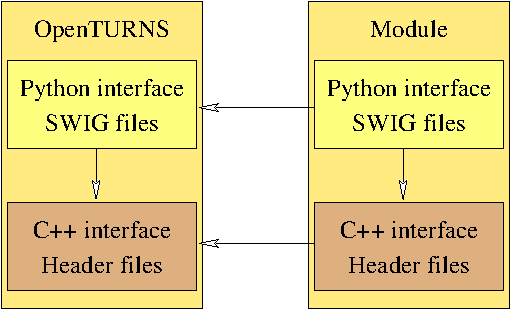
\includegraphics{OTModule.pdf}}
  \begin{block}{The principles}
    An OpenTURNS module is typically made of two parts:
    \begin{itemize}
    \item a C++ part that uses the OpenTURNS C++ interface in order to provide new specialization or to produce instances of the data model using new algorithms with no OpenTURNS counterpart.
    \item a Python part, the Python interface of the C++ part, often obtained using SWIG. In this case, this SWIG interface must use the OpenTURNS interface the same way its C++ interface uses the OpenTURNS C++ interface.
    \end{itemize}
  \end{block}
\end{frame}
\begin{frame}
  \frametitle{OpenTURNS modules}
  \begin{block}{And for a Python module?}
    For now, there is (almost) no way to use a Python object within the OpenTURNS C++ library, excepting:
    \begin{itemize}
    \item A Distribution;
    \item a Function;
    \item An experiment
    \item ...
    \end{itemize}
    and use these one as "OpenTURNS classes".\\
    The concept of "OpenTURNS Python module" is not very specific: we get some `full python` packages such as \texttt{oticp}, \texttt{otwrap} , \texttt{otsklearn}. But these examples are in a way independent as they rely on the "OpenTURNS API" and the API is not able to `integrate` them.
    In other words, any set of Python classes or Python functions that use the OpenTURNS Python interface can be called an OpenTURNS Python module. In this case, the notion of OpenTURNS module is mainly a packaging notion, and the use of the Python setup tools is probably more mature and more adapted!
  \end{block}
\end{frame}
\section[Module development]{Module development}
\begin{frame}
  \frametitle{Module development}
  \begin{block}{Step 1: copy and adapt an existing template}
    \begin{itemize}
    \item Copy and rename the source tree of an example module (for example the Strange module) from the OpenTURNS source tree. The examples modules are located under the module subdirectory of OpenTURNS source tree:\\

      {\ttfamily git clone https://github.com/openturns/ottemplate.git MyModule}
    \item Adapt the template to your module:\\
      {\ttfamily ./customize MyModule}\\
      This command change the module name into all the scripts, and adapt the example class to this new name.
    \end{itemize}
  \end{block}
\end{frame}

\begin{frame}
  \frametitle{Module development}
  \begin{block}{Step 2: develop the module}
    \begin{itemize}
    \item Implement your module. You are free to use the rules you want, but if the final objective of the module is to be integrated in the official release of OpenTURNS, it is wise to adopt the OpenTURNS development process and rules.
    \item Build your module as usual:
      \begin{tabular}{l}
        \ttfamily mkdir build\\
        \ttfamily cd build\\
        \ttfamily cmake .. -DCMAKE\_INSTALL\_PREFIX=INSTALLDIR \\
        \ttfamily -DOpenTURNS\_DIR=OPENTURNS\_INSTALLDIR/lib/cmake/openturns\\
        \ttfamily make
      \end{tabular}
    \item Create a source package of your module:\\
      {\ttfamily make dist}\\
      It will create a tarball named mymodule-X.Y.Z.tar.gz (and mymodule-X.Y.Z.tar.bz2), where X.Y.Z is the version number of the module.
    \end{itemize}
  \end{block}
\end{frame}


\begin{frame}
  \frametitle{Module development}
  \begin{block}{Step 3: documentation}
    Module documentation is very close to API one:
    \begin{itemize}
    \item Developer guide : Architecture, validation
    \item SWIG documentation is to be completed (docstrings); 
    \item Examples and API documentation;
    \item Theory (if needed)
    \end{itemize}
  \end{block}
\end{frame}


\begin{frame}
  \frametitle{Module development}
  \begin{block}{Step 4: install and test the module}
    \begin{itemize}
    \item Check that you have a working OpenTURNS installation, for example by trying to load the OpenTURNS module within an interactive python session:
      \begin{tabular}{l}
        \ttfamily python\\
        \ttfamily >>> import openturns as ot\\
      \end{tabular}
      and python should not complain about a non existing openturns module.
      The installation script has many more capabilities, you can access to its embedded documentation by invoking it without argument.
    \item Test your module within python:\\
      \begin{tabular}{l}
        \ttfamily python \\
        \ttfamily >>> import openturns as ot \\
        \ttfamily >>> import mymodule \\
      \end{tabular}
      and python should not complain about a non existing mymodule module.
    \end{itemize}
  \end{block}
\end{frame}


\begin{frame}
  \frametitle{Module development}
  \begin{block}{Step 5: Maintenance}
    Each developer is responsible of his package should maintain it!
    \begin{itemize}
    \item We can rely on continuous integration tool accounting API changes
    \item He is in charge of bugs (except if underlying bug is in the API)
    \end{itemize}
    Exception : modules maintained by the consortium!
  \end{block}
  
  \begin{block}{Step 6: Packaging}
    No specific rule concerning the packaging!
    \begin{itemize}
    \item Tarball generation
    \item Git
    \item conda...
    \end{itemize}
    Exception : modules maintained by the consortium!
  \end{block}
\end{frame}

\end{document}
